\documentclass[journal,comsoc]{IEEEtran}

\usepackage[T1]{fontenc}
\usepackage{amsmath}
\interdisplaylinepenalty=2500
\usepackage[cmintegrals]{newtxmath}
\usepackage{graphicx}
\graphicspath{{./figure/}}

\hyphenation{op-tical net-works semi-conduc-tor}

\begin{document}

\title{A Text Relating the Group Description}

\author{Cao Fei,~\IEEEmembership{Repository Manager,}
     He Ling,~\IEEEmembership{Data Manager,}
    Man Zhaolong,~\IEEEmembership{Bibliography Manager,}
   \\ and~Zhen Qi,~\IEEEmembership{Document Manager}}
 
 
 
 \markboth{Operational Statistics for SAR Imagery, October~2020}%
{Shell \MakeLowercase{\textit{et al.}}: Bare Demo of IEEEtran.cls for IEEE Communications Society Journals}


\maketitle

\IEEEpeerreviewmaketitle


\section{Members}
\IEEEPARstart{T}{here} are four members in our group. The introduction of each member is as follows.

\begin{IEEEbiography}[{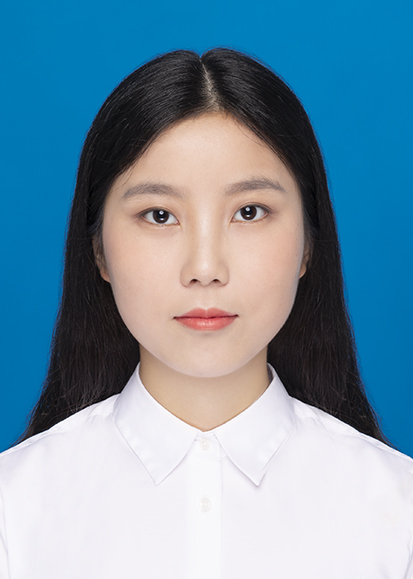
\includegraphics[width=1in,height=1.25in,clip,keepaspectratio]{figure//CaoFei.jpg}}]{Cao Fei}
(Repository Manager) received the degree of  Bachelor in Engineering in Communication Engineering from the China University Of Geosciences, wuhan, China, in 2020. She is studying for a Master degree in Computer Science and Technology in Xidian University.\\
\hspace*{0.2cm}During the undergraduate study, she has exposed to the knowledge of Machine Learning and Image Processing. Her future research field may be Semantic Segmentation and Object Detection out of interest.
\end{IEEEbiography}

\begin{IEEEbiography}[{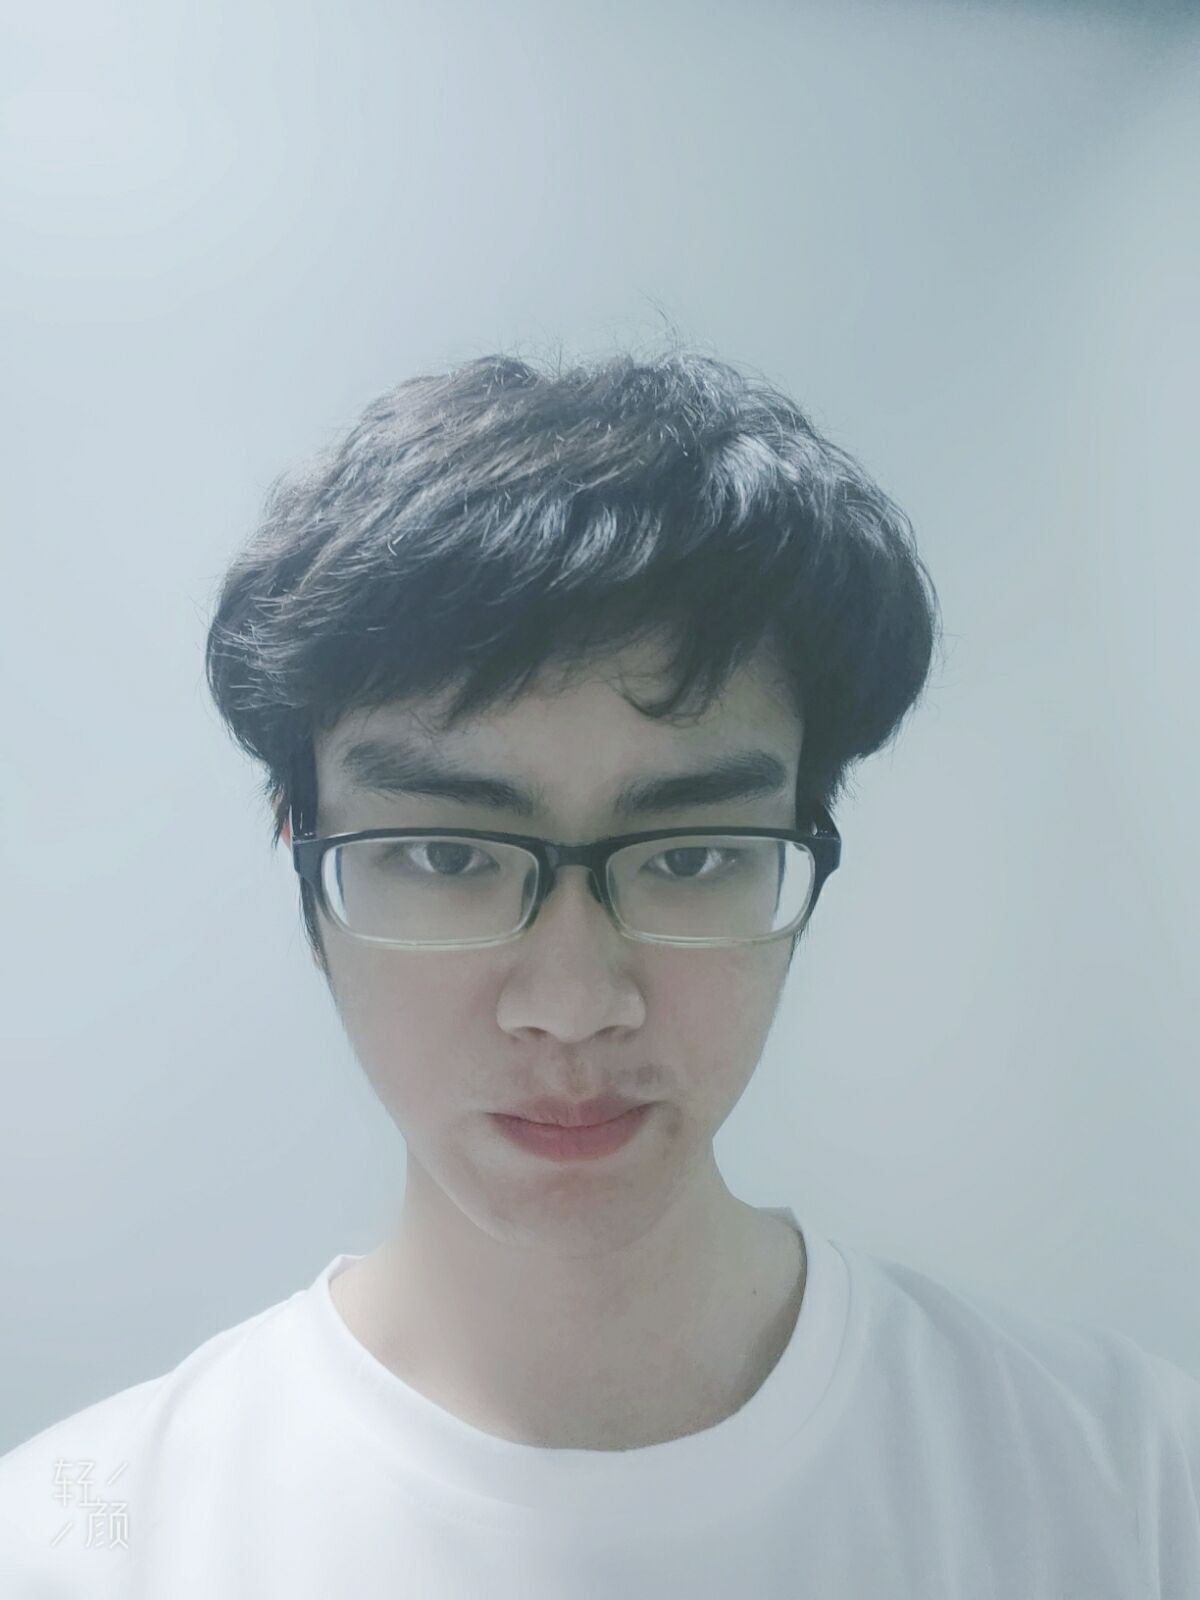
\includegraphics[width=1in,height=1.25in,clip,keepaspectratio]{figure//HeLing.jpg}}]{He Ling}
(Data Manager) received the degree of  Bachelor in Mechanical design, manufacturing and automation from XiDian University, xi'an, China, in 2020. He is studying for a Master degree in Electronic Information in Xidian University.\\
\hspace*{0.2cm}He is an excellent person with solid theoretical foundation and and practical ability. His current research area is Remote Sensing Images.
\end{IEEEbiography}

\begin{IEEEbiography}[{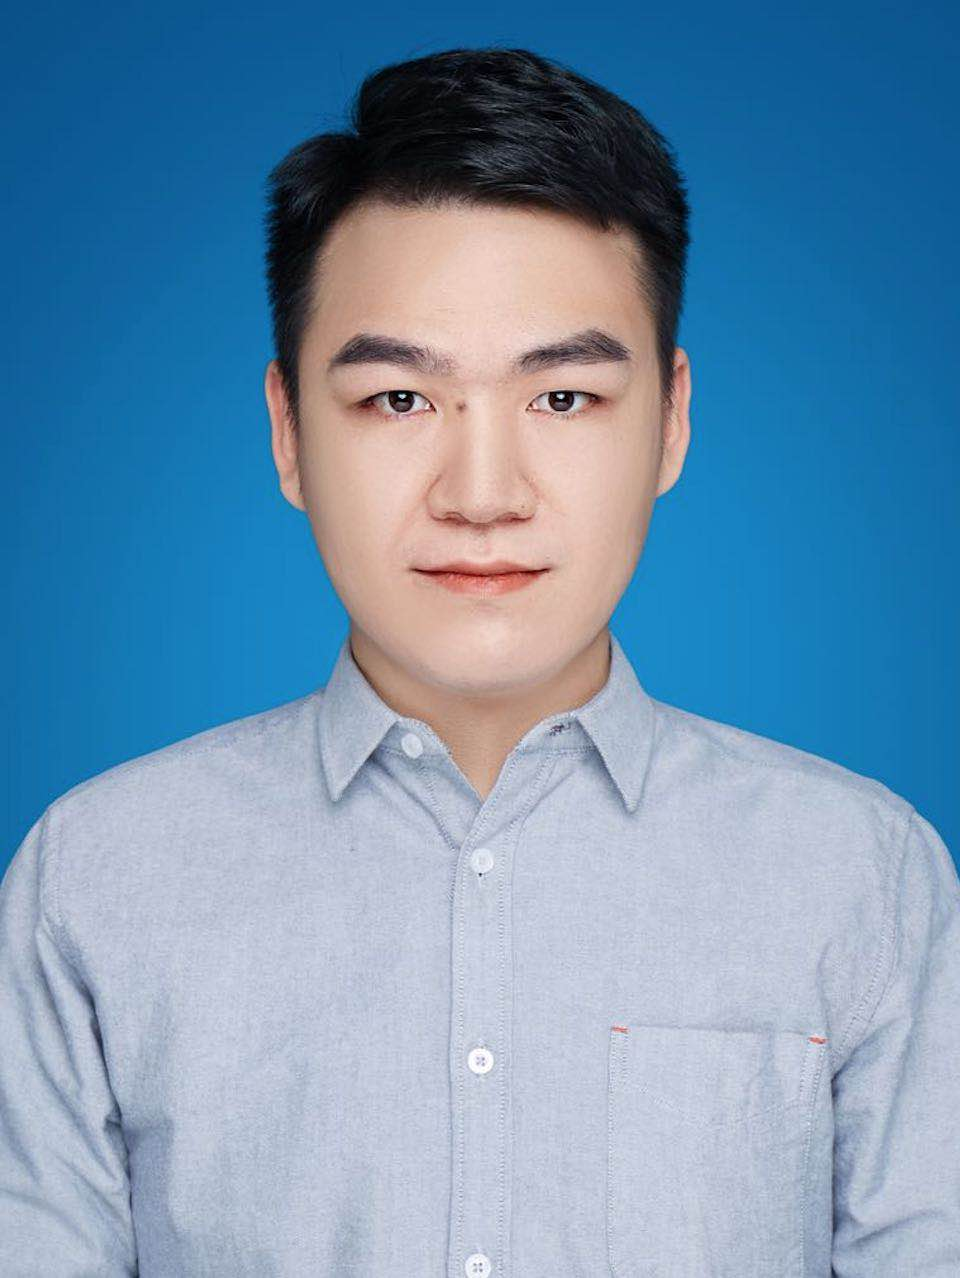
\includegraphics[width=1in,height=1.25in,clip,keepaspectratio]{figure//ManZhaolong.jpg}}]{Man Zhaolong}
(Bibliography Manager) received the degree  of Bachelor in Internet of Things from Anhui Agricultural University, Anhui, China, in 2018. He is studying for a Master degree in Electronic Information in Xidian University.\\
\hspace*{0.2cm}He is a good team player with a fantastic programming background. He is interested in Convolutional Neural Networks.
\end{IEEEbiography}


\begin{IEEEbiography}[{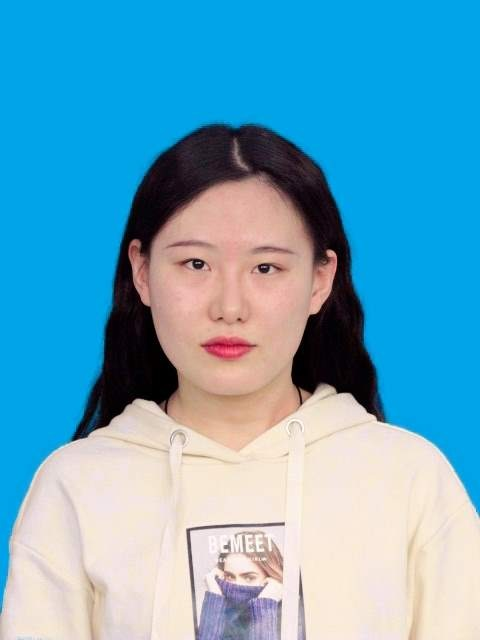
\includegraphics[width=1in,height=1.25in,clip,keepaspectratio]{figure//ZhenQi.jpg}}]{Zhen Qi}
(Document Manager) received the degree of  Bachelor in Statistics from XiDian University, xi'an, China, in 2020. She is studying for a Master degree in Electronic Information in Xidian University.\\
\hspace*{0.2cm}She is a cheerful and lively person and has a certain reserve of mathematical knowledge. Her future research feild may be Spectral clustering or Hyperspectral Image.
\end{IEEEbiography}


\end{document}

